\section{Overview}
\begin{figure}[t!]
    \centering
    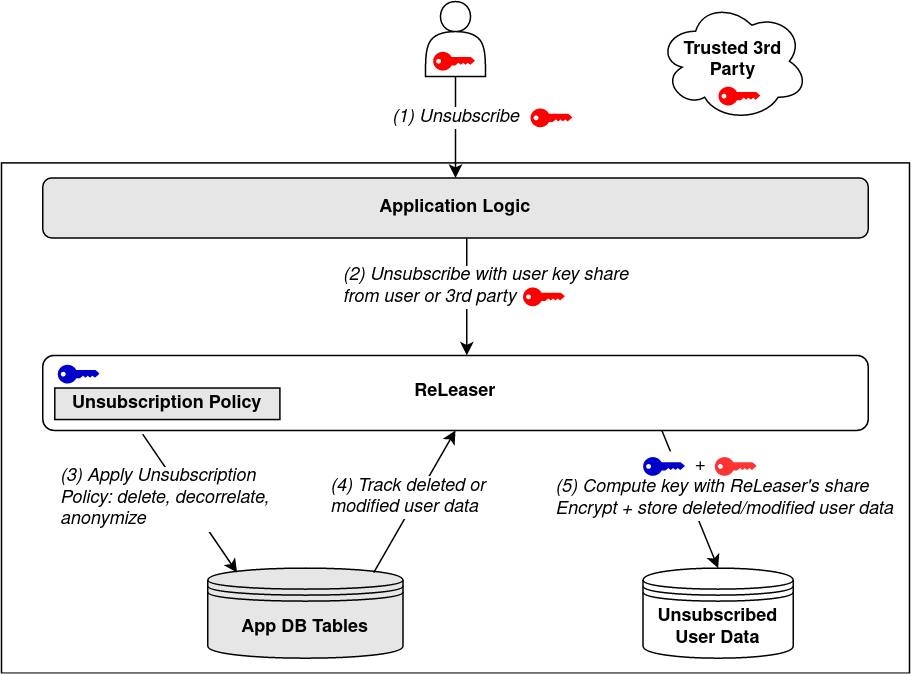
\includegraphics[width=0.5\textwidth]{img/releaser_arch}

    \caption{High-level \sys architecture. Developers specify the grayed-out components (app logic, DB table schema, and
    unsubscription policy).}
    \label{fig:arch}
\end{figure}

To solve these challenges, we present \sys, a system designed to achieve the \name paradigm.
As shown in Figure~\ref{fig:arch}, \sys sits between the application logic and the application database, adding support for
\texttt{UNSUBSCRIBE} and \texttt{RESUBSCRIBE} queries, and applying the appropriate data transformations
during unsubscription and resubscription.

\sys models application data as a graph of \emph{entity} nodes and edges, where each entity type
corresponds to an application datatable, such as a users, papers, or reviews table. Edges between
entities are foreign key relationships: foreign key table columns 
create child-parent correlations, where the child entity holds the
parent entity's identifier as a foreign key. 
%\sys also includes abstract entities in the graph, where the keys may be non-referential
%identifiers that refer to abstract, non-table entities (e.g.,\ a \texttt{thread\_id} column in the
%comments table).  
%Edges---foreign key relationships---represent correlations between the nodes (entities) of the
%graph.
%---foreign or abstract key relationships---

Developers use their application expertise to determine an appropriate post-unsubscription state,
specifying how entities and edges should be modified to achieve both de-identification and application correctness. 
\sys provides a menu of choices for removing or modifying entity content and edges (Section~\ref{sec:design:unsub}).
Developers reason only about the \emph{types} of entities and the \emph{types} of entity edges
in the application schema, while \sys acts on individual instances of the resulting entity graph. \sys and
ensures that unsubscription achieves the state specified in the policy, and can be reversed upon
resubscription. 
The unsubscription policy can also act as a specification of
application database state to precisely convey privacy guarantees to users.

\sys also handles user data management and storage.
While unsubscribing a user, \sys tracks all deletions and modifications to the database. 
\sys encrypts this log with a per-user key, and stores this encrypted
blob in a dedicated application datastore (Figure~\ref{fig:arch}, step 5). The user key is secret-shared using a (2, 3)
threshold scheme~\cite{secretsharing} between the user, \sys, and a trusted third party (\eg
Amazon S3), so that the user can authorize \sys and the third party to restore the key if
the user forgets their share. 
%Alternatively, the key can also be password-encrypted, which relies
%on the user not forgetting their password.
The user can optionally choose to store this encrypted data themselves 
%(or in a third party cloud provider), 
and be in charge of providing their data and key to \sys to decrypt the data upon
resubscription.

To resubscribe, a user authorizes the decryption of their data and associated metadata by
providing their share of the key (or authorizing a trusted third party to reconstruct the secret
with the application). \sys decrypts the data with the key, and systematically reverses 
the modifications made during unsubscription, restoring removed entities and correlations between
entities.

%%%%%%%%%%%%%%%%%%%%%%%%%%%%%%%%%%%%%%%%%%%%%%%%%%%%%%%%%%%%%%%%%%%%%%%%%%%%%%%%%%%%%%%%%%%%%%%%%%%%%%
%%%%%%%%%%%%%%%%%%%%%%%%%%%%%%%%%%%%%%%%%%%%%%%%%%%%%%%%%%%%%%%%%%%%%%%%%%%%%%%%%%%%%%%%%%%%%%%%%%%%%%
%%%%%%%%%%%%%%%%%%%%%%%%%%%%%%%%%%%%%%%%%%%%%%%%%%%%%%%%%%%%%%%%%%%%%%%%%%%%%%%%%%%%%%%%%%%%%%%%%%%%%%

\iffalse
With \sys, developers write an \emph{unsubscription policy} that specifies the high-level,
post-unsubscription state of application data.  The policy indicates how the database contents need
to change to meet de-identification requirements on user unsubscription, while still retaining data
necessary for the application to function. \sys then turns this policy into a set of concrete,
executed database operations that prototematically remove, anonymize, and structurally
\emph{decorrelate} user data upon unsubscription to meet the resulting spec. \sys 
encrypts decorrelated or removed user data with a user-specific key, which can be either
password-encrypted by the application, or secret shared~\cite{secretsharing} with a trusted third
party. \sys provides a way for the application to store the encrypted blob, and deletes the plaintext
data.

\sys's policy abstractions require knowledge of only the application schema and the high-level
application's semantics. Using these abstractions, developers pinpoint how identifying information
leaks either (1) directly via data content, or (2) indirectly via the structural \emph{correlations}
(foreign key relationships) between data records. Developers use their application expertise to
select from a set of policy choices that alter these contents and correlations, choosing the policy
that provides the greatest amount of de-identification while still preserving application
utility and correctness.

When a user resubscribes, \sys decrypts and inserts missing data, automatically
\emph{recorrelating} the data with the user account and restoring the user to her
original subscribed state as much as possible.
\fi
